\subsubsection{Cơ sở lý thuyết}
Sau khi đọc những tài liệu về Machine Learning và Deep Learning, nhóm của chúng em đã quyết định chọn thuật toán \textbf{Gradient Descent} để giải quyết bài toán này. Và sau đây là lý do chúng em chọn thuật toán này.

Ở đây, ta quay lại với một thuật toán vô cùng phổ biến \textbf{Linear Regression} (Hồi quy tuyến tính). Nhóm cũng đã thực hiện thuật toán này cho BTL môn Cấu trúc rời rạc cho KHMT trong kì trước. Bây giờ ta hãy cùng xem xét lại thuật toán Linear Regression nhiều biến.

Hàm mất mát của thuật toán là:
$$J(w) = \frac{1}{2m} \sum_{i=1}^{m} ( \widehat{y}^{(i)} - y^{(i)}) ^{2}$$
$$= \frac{1}{2m} \sum_{i=1}^{m} ( wx^{(i)} - y^{(i)}) ^{2}$$
$$= \frac{1}{2m} \parallel Xw - y \parallel ^{2}$$

$$w=\begin{bmatrix}w_{0} \\ w_{1} \\ … \\ w_{n} \end{bmatrix}, X= \begin{bmatrix}1 & x_{1}^{(1)} & … & x_{n}^{(1)} \\1 & x_{1}^{(2)} & … & x_{n}^{(2)} \\… & … & … & … \\1 & x_{1}^{(m)} & … & x_{n}^{(m)}\end{bmatrix}, y=\begin{bmatrix}y^{(1)} \\ y^{(2)} \\ … \\ y^{(m)} \end{bmatrix}$$
Nhiệm vụ của ta là tìm vector $w$ sao cho hàm mất mát $J(w)$ nhỏ nhất.

Bằng phương pháp của Giải tích, ta tính \textbf{đạo hàm riêng} theo từng biến $w_{0}, w_{1}, …, w_{n}$ giải hệ các đạo hàm riêng bằng 0 và tìm được nghiệm
$$w = (X^{T}X)^{+}X^{T}y$$

Thế nhưng, ở đây ta bắt gặp 2 vấn đề đối với thuật toán này:
\begin{enumerate}
    \item Thứ nhất, nếu m và n lớn thì các ma trận và vector trên sẽ rất lớn. Điều này không những tốn bộ nhớ mà quá trình tính toán còn trở nên chậm chạp. Nếu m, n không quá lớn, công thức trên là cách đơn giản nhất để giải quyết bài toán, ngược lại, ta sẽ cần một cách khác tối ưu hơn.
\item  Thứ hai, khi khảo sát hàm mất mát, để tìm điểm cực tiểu ta giải hệ các đạo hàm riêng bằng 0. Đối với phương trình tuyến tính việc này rất đơn giản và ta tìm ra được nghiệm như trên. Nhưng trong nhiều thuật toán, hàm mất mát phức tạp hơn và cách giải đó trở nên quá khó hoặc bất khả thi. Ta cần phương pháp tổng quát hơn để tìm điểm cực trị của hàm bất kỳ, hay trong trường hợp này là tìm cực tiểu.
\end{enumerate}

Thuật toán Gradient Descent giải quyết cả hai vấn đề trên và cũng mang tính tổng quát về toán học hơn.

{\large\textbf{Thuật toán Gradient Descent}}
\begin{itemize}
    \item Thuật toán Gradient Descent dùng để tìm điểm cực trị của hàm số. Đối với nhiều hàm số, việc khảo sát bằng cách tính đạo hàm rất khó khăn hoặc bất khả thi, Gradient Descent cung cấp một phương thức tổng quát cho những trường hợp này. 
    \item Ta xem xét hiện tượng sau: Quả bóng đang lăn xuống dốc. Trong một môi trường, quả bóng lăn xuống càng nhanh khi dốc càng đứng (mặc dù không phải vậy) và khi xuống đến chân dốc thì quả bóng dừng lại. Hiện tượng này rất dễ hình dung và giúp ta hiểu tư tưởng của Gradient Descent.
    \begin{figure}[H]
        \centering
        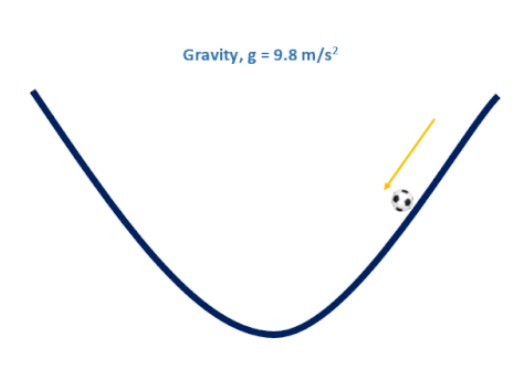
\includegraphics[width=0.5\textwidth]{image/bt5/lt_vd.jpg}
    \end{figure}

    \item Xét hàm số $y = f(x)$ và ta cần tìm điểm cực tiểu của hàm số.
    \item Xuất phát từ điểm x bất kỳ, ta cần điều chỉnh x để nó có xu hướng tiến về điểm mà hàm số đạt cực tiểu. Điều này có thể đạt được bằng cách lặp lại liên tiếp phép biến đổi: $x = x - \alpha f’(x)$
        \begin{figure}[H]
        \centering
        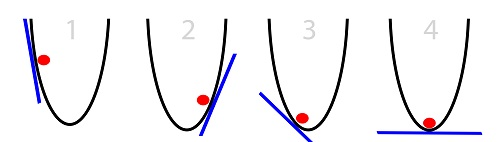
\includegraphics[width=0.5\textwidth]{image/bt5/lt_mh.jpg}
        \end{figure}
     \item Thông thường, ta không thể thực hiện phép lặp đến khi $f'(x) = 0$ được mà khi $|f'(x)|$ rất nhỏ ta coi như đã tìm được điểm cực tiểu.
     \item Trong phép biến đổi trên, $\alpha$ được gọi là \textbf{learning rate}. \textbf{Learning rate} càng lớn thì mỗi “bước nhảy” của x sẽ càng lớn và số lần lặp cần thiết để tìm được điểm cực tiểu sẽ giảm đi. Tuy nhiên nếu learning rate quá lớn thì có thể sau mỗi lần lặp x càng cách xa điểm cực tiểu và ta không thể tìm được điểm cực tiểu.
        \begin{figure}[H]
        \centering
        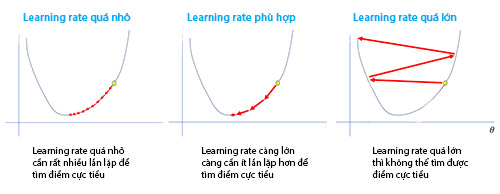
\includegraphics[width=0.7\textwidth]{image/bt5/lt_rate.jpg}
        \end{figure}
     \item Vì lý do đó việc chọn \textbf{learning rate} phù hợp là rất quan trọng. Ta có thể thử nhiều giá trị \textbf{learning rate} khác nhau để tìm ra giá trị \textbf{learning rate} đủ tốt.
     \item \textbf{Lưu ý: } Thuật toán Gradient Descent dùng để tìm ra điểm mà hàm số đạt cực tiểu chứ không phải đạt giá trị nhỏ nhất. Đối với hàm số có nhiều cực tiểu thì tùy thuộc vào vị trí điểm chọn ban đầu, ta có thể tìm được kết quả khác nhau. 
        \begin{figure}[H]
        \centering
        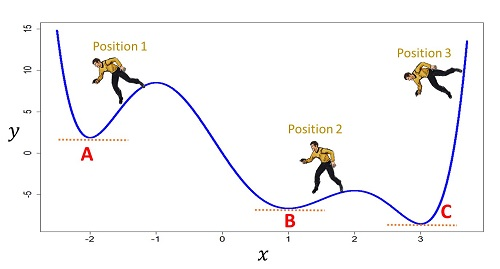
\includegraphics[width=0.7\textwidth]{image/bt5/lt_rateah.jpg}
        \end{figure}
    Hình trên minh họa cho ảnh hưởng của điểm ban dầu với kết quả của Gradient Descent. Nếu ta xuất phát từ vị trí thứ nhất thì thuật toán sẽ dừng lại khi di chuyển đến A, nếu xuất phát từ vị trí thứ hai thì thuật toán dừng lại tại B, nếu xuất phát từ vị trí thứ ba thì thuật toán dừng lại tại C.
    \item \textbf{Nhận xét:} Đối với công thức \textbf{Explicit Euler}, thật may mắn khi hàm mất mát của nó khi ta biến đổi chỉ có một cực tiểu. Do đó ta có thể dùng Gradient Descent kết hợp Explicit Euler để tìm điểm cực tiểu đó cũng chính là điểm mà hàm mất mát đạt giá trị nhỏ nhất. Đây chính xác là những gì chúng ta sẽ làm ở bài toán dự đoán này!
\end{itemize}
{\large\textbf{Áp dụng vào bài toán}}

\begin{itemize}
    \item Hàm mất mát (cost function) bằng một nửa trung bình cộng bình phương các khoảng cách sai lệch trong hình dưới đây.
     \begin{figure}[H]
        \centering
        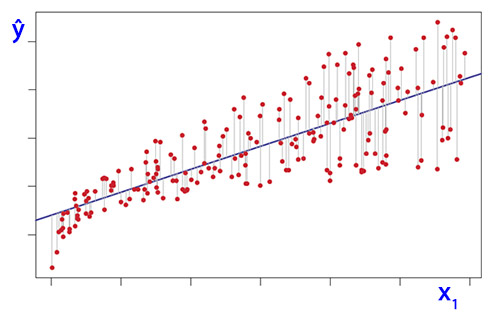
\includegraphics[width=0.7\textwidth]{image/bt5/lt_cost.jpg}
        \end{figure}
        $$J= \frac{1}{2m} \sum_{i=1}^{m} ( X_{predict}^{(i)} - X_{exact}^{(i)}) ^{2}$$
        trong đó m là số input ban đầu được dùng để đào tạo thuật toán
        \item Nếu thắc mắc tại sao chỉ lấy một nửa $\frac{1}{2m}$, đó là do khi khảo sát hàm mất mát, việc lấy đạo hàm của một bình phương sẽ phải nhân hệ số 2 và nó sẽ bù trừ cho $\frac{1}{2}$ giúp đạo hàm trở nên đơn giản hơn.
        \item Với bài toán của chúng ta, $m=1000$, là tập dữ liệu tình yêu của Romeo và Juliet dành cho đối phương. Hàm mất mát của ta bấy giờ sẽ là:
        $$J_{X}=\frac{1}{2*1000} \sum_{i=1}^{1000} ( X_{predict}^{(i)} - X_{exact}^{(i)}) ^{2}$$
        với $X=\begin{pmatrix}
        R\\ T
\end{pmatrix}$
        \item Biến đổi theo công thức \textbf{Explicit Euler} ở bài tập 4, ta được Cost function lúc này là:
        $$\left\{\begin{matrix}
J_R= & \frac{1}{2*1000} \sum_{i=1}^{1000} ( (R_{0}+h(aR_{0}+bJ_{0}))^{(i)} - R_{exact}^{(i)}) ^{2} \\ 
J_J= & \frac{1}{2*1000} \sum_{i=1}^{1000} ( (J_{0}+h(cR_{0}+dJ_{0}))^{(i)} - J_{exact}^{(i)}) ^{2}
\end{matrix}\right.$$
    \item Các bước áp dụng thuật toán:
    \begin{enumerate}
        \item Chọn 1 giá trị learning rate $\alpha$ và xuất phát từ một điểm được chọn bất kỳ (a,b,c,d)
        \item Liên tiếp lặp lại phép biến đổi:
            $\left\{\begin{matrix}
a = a-\alpha J'_{a}\\ 
b= b-\alpha J'_{b}\\ 
c= c-\alpha J'_{c}\\ 
d= d-\alpha J'_{d}\\ 
\end{matrix}\right.$
        \item Thuật toán dừng lại khi cost function $J$ thay đổi rất nhỏ hoặc hay nói cách khác $J$ hội tụ. Nếu thuật toán không thể kết thúc thì ta tiếp tục chọn giá trị $\alpha$ nhỏ hơn rồi quay lại bước 2.
    \end{enumerate}
        

\end{itemize}
\subsubsection{Hiện thực và kết quả dự đoán}
\par Code xây dựng mô hình cũng như dự đoán kết quả đồ thị chi tiết nằm ở đường link sau: \href{https://colab.research.google.com/drive/1m0rewA-U1Gx6qWTZARUoIuVBGPOEghOZ?fbclid=IwAR2-uZabt8mZ7-FcAazQpRfiNmZ_KHRS_BkDiebGcHR5oiK1Hybkb-wkDyE#scrollTo=_75wYhU5HtCe}{Exercise 5} hoặc nằm ở trong file \textit{Pro5.py} trong bài nộp tập tin nén. 
\newline
Trong quá trình xây dựng mô hình, nhóm chọn được \textit{learing rate} thích hợp nhất mang giá trị là 3.5 và số lần lặp của phép biến đổi là 3500 để cho ra được đồ thì của Romeo và Juliet khớp (fit) với dữ liệu nhất có thể. Hình sau là output của của mô hình dự đoán được về giá trị của $a, b, c, d$, giá trị hàm mất mát của mô hình dự đoán được và đồ thị của tình yêu Romeo và Juliet: 
\begin{figure}[H]
    \centering
    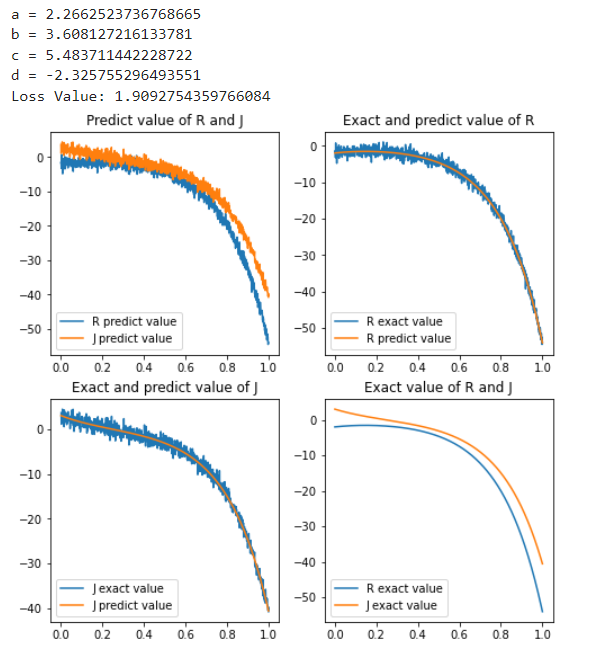
\includegraphics[width=0.7\textwidth]{image/bt5/Output Model.png}
    \caption{Giá trị các hệ số dự đoán và đồ thị tình yêu của Romeo và Juliet}
\end{figure}
Theo trong hình, ta có thể thấy giá trị các hệ số \textit{(làm tròn)} tính ra được xấp xỉ là $a = 2.2663, b = 3.6081, c = 5.4837, d = -2.3258$, với R là tình yêu của Romeo, J là tình yêu của Juliet. 
\newline
\newline
Để làm rõ tính tin cậy của các hệ số tính ra, nhóm cũng trực quan hóa giá trị của hàm mất mát \textit{cost function} theo từng vòng lặp trong phép biến đổi. Để mang tính chính xác hơn do chêch lệch thay đổi của hàm mất mát khá lớn giữa các vòng lặp, nhóm sẽ vẽ đồ thị của giá trị \textcolor{blue}{$\log (cost \: function \: value)$} : 
\begin{figure}[H]
    \centering
    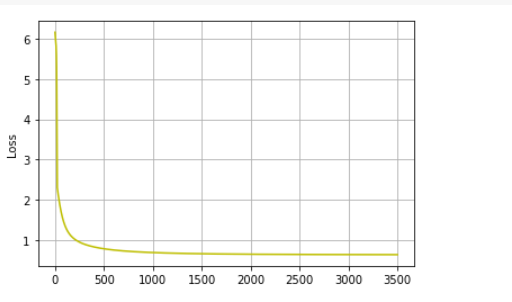
\includegraphics[width=0.7\textwidth]{image/bt5/Loss Func plot.png}
    \caption{Đồ thị giá trị của cost function theo số lần thực hiện vòng lặp biến đổi}
\end{figure}
Ta có thể thấy rằng giá trị của hàm mất mát hội tụ dần về một giá trị và hầu như không đổi khi số vòng lặp biến đổi từ 2000 trở đi. Vậy ta có thể kết thúc thuật toán và đảm bảo về độ tin cậy của giá trị các hệ số dự đoán được.
\newline
\newline
{\large\textbf{Kết luận}}
\newline
Vậy nhóm kết luận giá trị dự đoán xấp xỉ của các hệ số là: $a = 2.2663, b = 3.6081, c = 5.4837, d = -2.3258$. \\
\\



      



























